% !TEX root = ../a1.tex

\section{Introduction}
In this report, we discuss the time complexity of six types of different sort algorithms including Bubble sort, Insertion sort, Selection sort, Merge sort and two types of Quick sorts, by testing their runtime with input in different sizes. The graph of time-size relationship intuitively demonstrates the time complexity, thus confirming our theoretical expectation.

Furthermore, this report entails several extreme situations like an integer array in descending order or an array of merely 1's. The result, interestingly, reflects the capacity of those six algorithms under different circumstances.

Since the time complexity of $O(n^2)$ and $O(n\log n)$ differs enormously with the increasing of input size, we separate the analysis into two parts and discuss respectively.

\section{Performance analysis on $O(n^2)$ Sort Algorithms}
\begin{figure}[H]
    \centering
    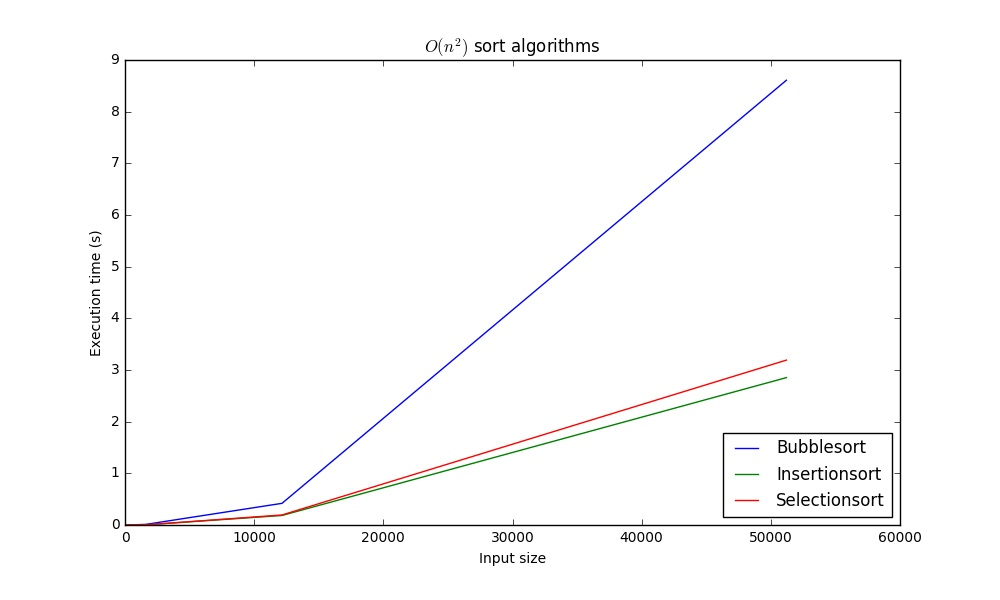
\includegraphics[width=0.8\linewidth]{../a1/012}
    \caption{Performance of $O(n^2)$ sort algorithms}\label{012}
\end{figure}
In Fig. \ref{012}, the curves are in shape of quadratic functions, among which the Bubble sort obtains a obvious larger constant. The runtime is considerably increasing non-linearly after the input size exceeds 25000.

\section{Performance analysis on $O(n\log n)$ Sort Algorithms}
\begin{figure}[H]
    \centering
    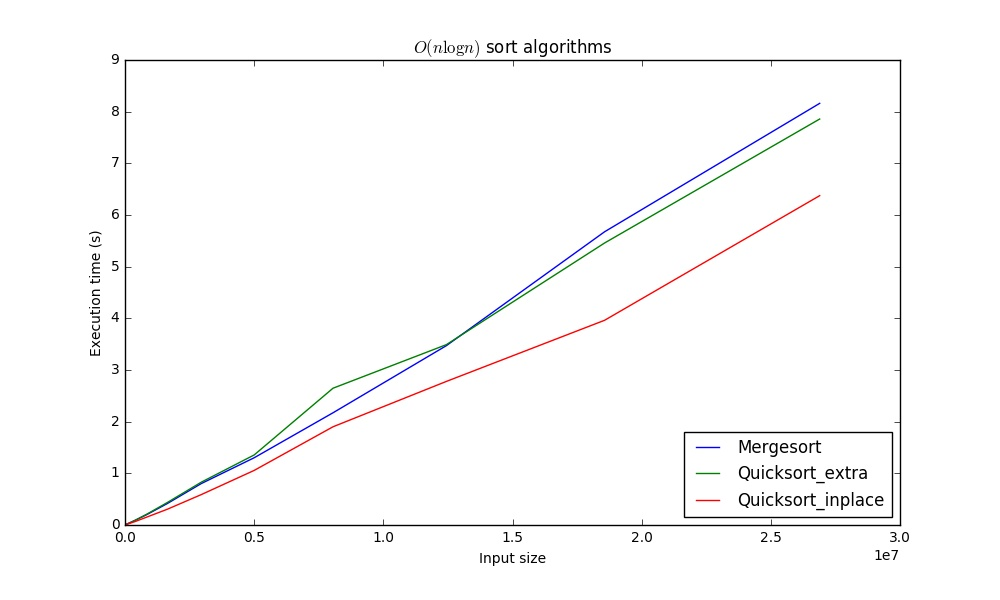
\includegraphics[width=0.8\linewidth]{../a1/345}
    \caption{Performance of $O(n\log n)$ sort algorithms}\label{345}
\end{figure}
In Fig. \ref{345}, the curves are almost linear, where the in-place Quick sort shows an undebatable edge. It's hard to tell whether it's $O(n\log n)$ or $O(n)$ because the input size is not large enough to give credit to the expectation. The distinction between two different Quick sort is intriguing. They followed almost the same procedure whereas a big gap occurred when even the input data is random. This reflects It also indicates that the randomized Quick sort works remarkably, even compared to other steady $O(n\log n)$ algorithms like Merge sort.

\section{Extreme Input Situations}
\subsection{An Array in Descending Order}
For descending data, we can see that Quick sort in-place is still advantageous, although all of them become more efficient. One possible explanation is that the descending data simultaneously reduces the cost on comparison between two elements. 
\begin{figure}[H]
    \centering
    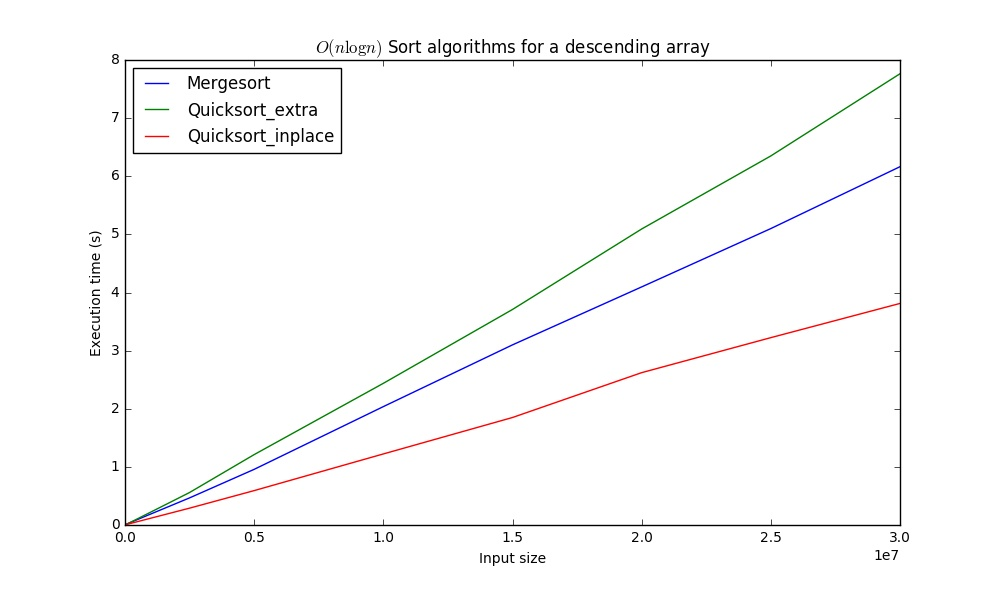
\includegraphics[width=0.8\linewidth]{../a1/reverse}
    \caption{Performance of $O(n\log n)$ sort algorithms}\label{345}
\end{figure}

\appendix
\section{Source Codes}
\inputcode{c++}{../a1/a1_test.cpp}{Sort algorithms}{1}
\inputcode{python}{../a1/test.py}{Test case generator}{2}
\inputcode{bash}{../a1/test.sh}{Cases runner}{3}
\inputcode{python}{../a1/plot.py}{Plotting program}{4}